% =====================================================================
%  Chapitre 2 -- partie c : qualite, jointures, imputation avancee
%  Densification (Licence 3 SDIA)
% =====================================================================

\begin{frame}{Le type d'une variable décide de tout}
\begin{center}
\small
\begin{tabular}{@{}p{0.17\textwidth}p{0.26\textwidth}p{0.36\textwidth}@{}}
\toprule
\textbf{Type} & \textbf{Exemple} & \textbf{Opérations autorisées} \\
\midrule
Nominale & filière, région & compter, regrouper ; \textbf{pas} d'ordre ni de
moyenne \\
Ordinale & niveau faible/moyen/élevé & comparer, ordonner ; pas de distance \\
Intervalle & température en °C & différences, moyenne ; pas de rapport \\
Ratio & revenu, âge & tout : sommes, rapports, moyenne \\
\bottomrule
\end{tabular}
\end{center}
\vspace{1.5mm}
\begin{wbox}[L'erreur de débutant]
Calculer une moyenne sur un code postal, ou une distance entre « faible » et
« élevé ». Le nombre existe, mais il ne veut rien dire : c'est un
\textbf{encodage}, pas une mesure.
\end{wbox}
\end{frame}

\begin{frame}{Explorer avant de modéliser}
\begin{center}
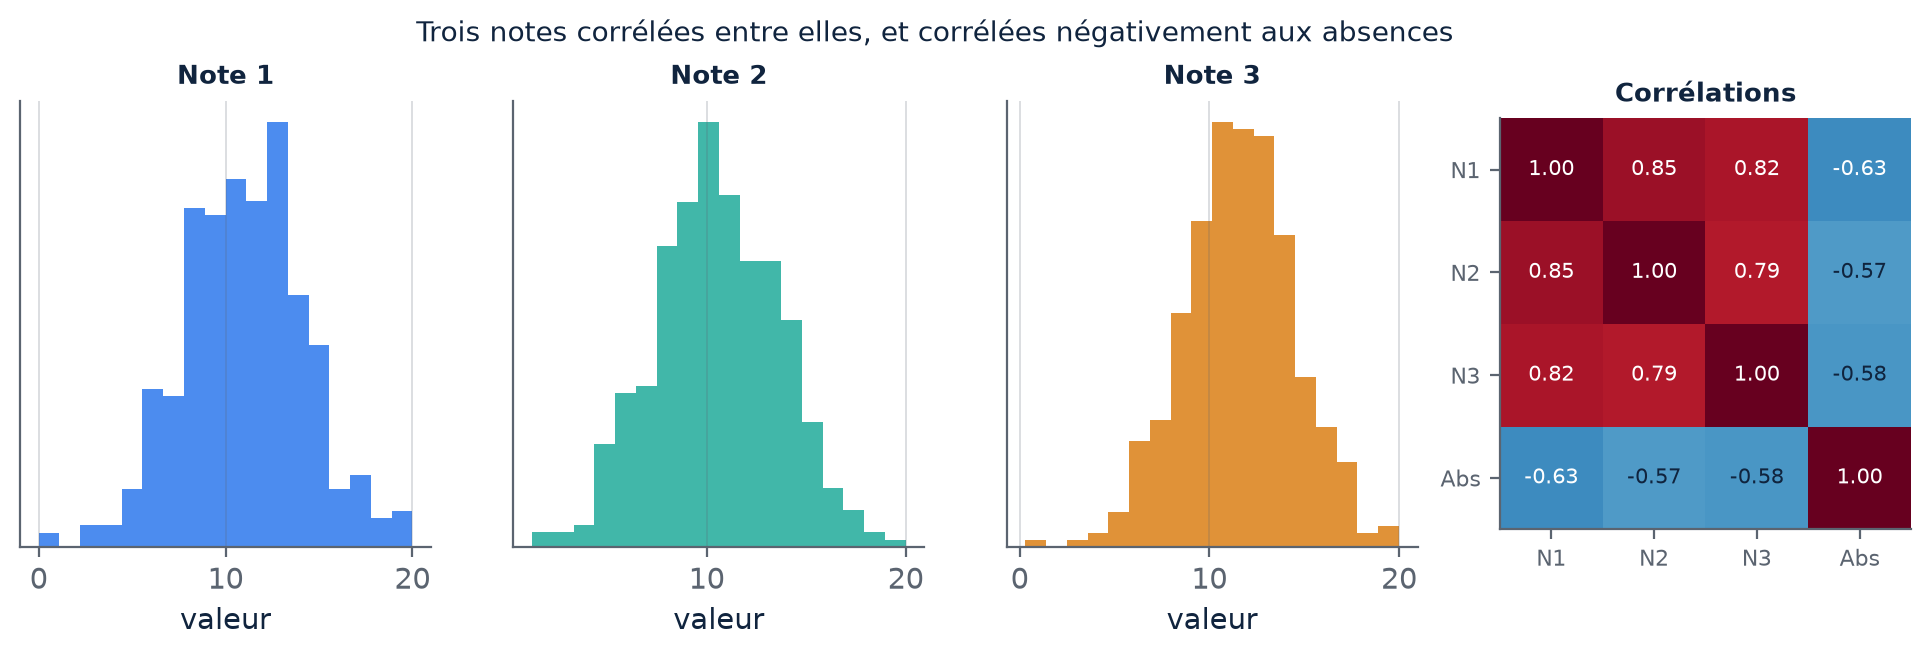
\includegraphics[width=0.95\textwidth]{h08_exploration.png}
\end{center}
\vspace{1mm}
\begin{columns}[t]
\begin{column}{0.48\textwidth}
\footnotesize
Les trois notes sont fortement corrélées : $r = 0{,}85$ entre la première et
la deuxième. Elles mesurent en partie \textbf{la même chose}.
\end{column}
\begin{column}{0.48\textwidth}
\footnotesize
Les absences sont corrélées négativement aux notes : $r = -0{,}63$ avec la
première. Signal utile, mais \textbf{corrélation n'est pas causalité}.
\end{column}
\end{columns}
\end{frame}

\begin{frame}{Redondance et multicolinéarité}
\begin{columns}[t]
\begin{column}{0.48\textwidth}
\begin{itemize}
  \item Deux colonnes corrélées à $0{,}85$ apportent presque la même
        information.
  \item Sur un modèle linéaire, les coefficients deviennent instables :
        un petit changement de données les fait changer de signe.
  \item Sur un modèle à arbres, l'importance se dilue entre les deux.
\end{itemize}
\end{column}
\begin{column}{0.48\textwidth}
\begin{kbox}[Que faire]
\begin{itemize}
  \item garder une seule des deux colonnes ;
  \item ou les combiner (moyenne, ACP) ;
  \item ou accepter la redondance et renoncer à interpréter les coefficients.
\end{itemize}
\end{kbox}
\end{column}
\end{columns}
\vspace{1mm}
\begin{wbox}[Ne pas confondre]
Redondance $\neq$ fuite. Deux colonnes corrélées dégradent l'interprétation ;
une fuite fabrique un score. Les deux se détectent à l'exploration.
\end{wbox}
\end{frame}

\begin{frame}{Qualité et provenance : les questions à poser}
\begin{center}
\small
\begin{tabular}{@{}p{0.26\textwidth}p{0.58\textwidth}@{}}
\toprule
\textbf{Question} & \textbf{Pourquoi elle compte} \\
\midrule
Qui est dans les données ? & un échantillon non représentatif produit un
modèle qui ignore une population entière \\
Sur quelle période ? & une année exceptionnelle (crise, grève) fausse la
relation apprise \\
Comment ont-elles été collectées ? & capteur, déclaratif et saisie manuelle
n'ont pas les mêmes erreurs \\
Y a-t-il des doublons ? & un même individu compté trois fois pèse triple dans
l'entraînement \\
Que signifie chaque colonne ? & une unité mal comprise (heures ou jours)
invalide tout le chapitre \\
\bottomrule
\end{tabular}
\end{center}
\vspace{1mm}
\begin{kbox}[Le réflexe]
Un jeu de données sans documentation se traite d'abord, se modélise ensuite.
Demander le dictionnaire des variables fait partie du travail.
\end{kbox}
\end{frame}

\begin{frame}{La jointure qui multiplie les lignes}
\vspace{1mm}
\begin{columns}[t]
\begin{column}{0.46\textwidth}
\centering
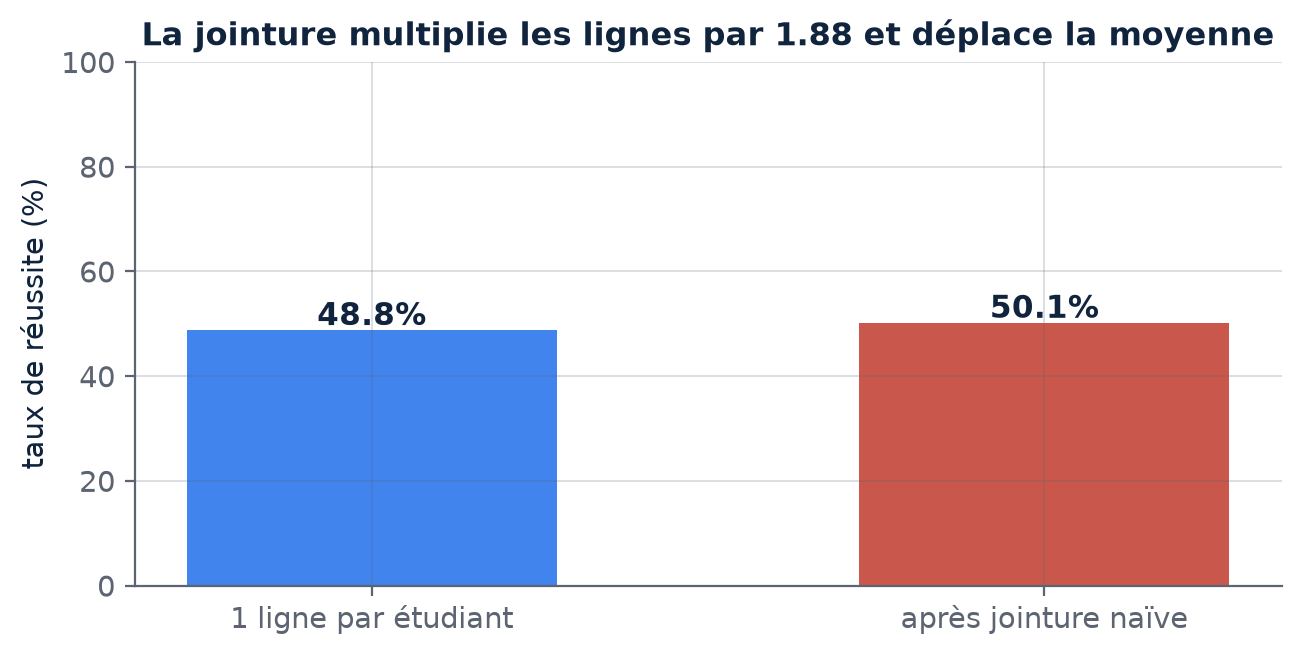
\includegraphics[width=\textwidth]{h09_jointure.png}
\begin{kbox}[Pourquoi]
La clé n'est pas unique à droite : la ligne de gauche est dupliquée.
\end{kbox}
\end{column}
\begin{column}{0.52\textwidth}
\begin{itemize}
  \item 400 étudiants, mais \textbf{752 lignes} après jointure.
  \item Facteur \textbf{1,88} : certains étudiants apparaissent 3 fois.
  \item Le taux de réussite passe de $48{,}7\,\%$ à $50{,}1\,\%$
        (\textbf{+1,4 point}) sans qu'aucune donnée n'ait changé.
\end{itemize}
{\footnotesize\color{byGrey}Toute statistique calculée après la jointure est
déplacée : agréger avant, ou pondérer.}
\end{column}
\end{columns}
\end{frame}

\begin{frame}{Avant de joindre : vérifier la cardinalité}
\begin{enumerate}
  \item Compter les lignes \textbf{avant} et \textbf{après} : le rapport doit
        être expliqué.
  \item Vérifier l'unicité de la clé de gauche
        (\py{df.duplicated(subset=cle).sum()}).
  \item Décider de l'agrégation : une ligne par individu (moyenne, dernière
        valeur, maximum).
  \item Contrôler les clés non appariées : jointure interne ou externe ?
  \item Recalculer les statistiques descriptives après la jointure.
\end{enumerate}
\vspace{1.5mm}
\begin{kbox}[Règle]
Une jointure n'est jamais neutre. Si le nombre de lignes change, la
distribution change, et tout ce qui suit change.
\end{kbox}
\end{frame}

\begin{frame}{Imputer mieux que par la moyenne}
\begin{columns}[t]
\begin{column}{0.46\textwidth}
\centering
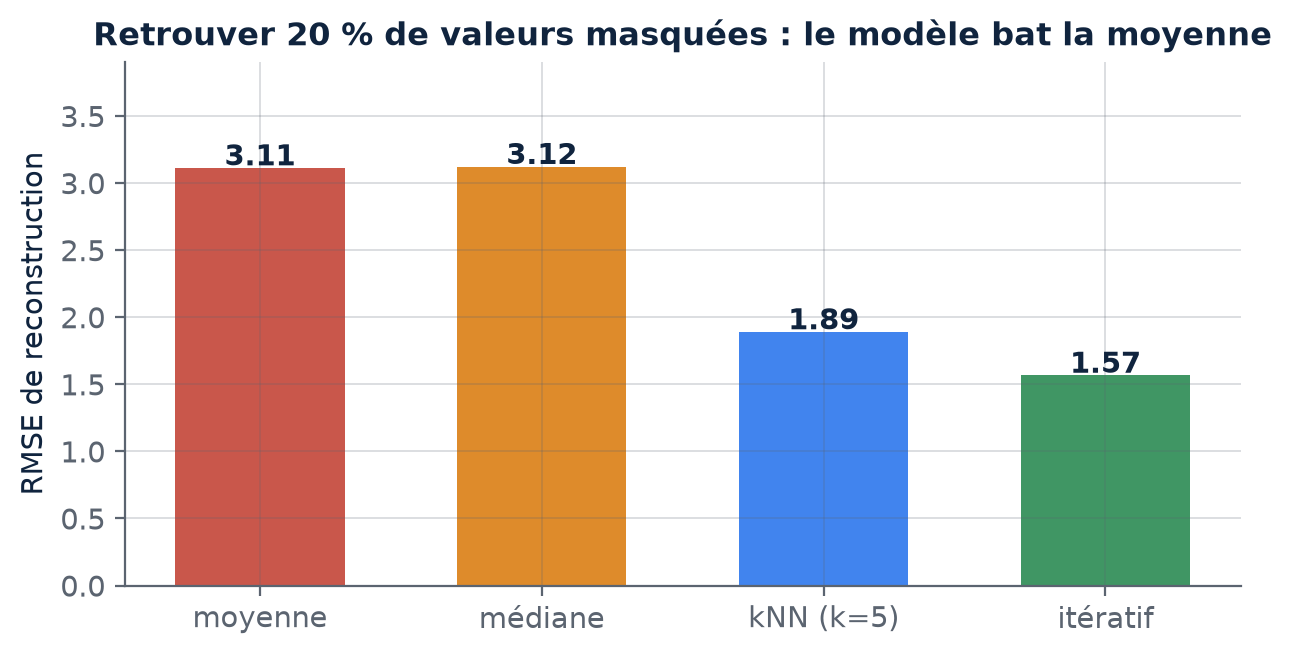
\includegraphics[height=0.34\textheight,keepaspectratio]{h10_imputations.png}
\end{column}
\begin{column}{0.52\textwidth}
\small
\begin{tabular}{@{}lr@{}}
\toprule
\textbf{Méthode} & \textbf{RMSE} \\
\midrule
Moyenne & $3{,}11$ \\
Médiane & $3{,}12$ \\
kNN ($k=5$) & $1{,}89$ \\
Itératif & $\mathbf{1{,}57}$ \\
\bottomrule
\end{tabular}
\vspace{2mm}
\begin{kbox}[Pourquoi les modèles gagnent]
Les trois notes sont corrélées : connaître deux notes renseigne la troisième.
La moyenne ignore cette information, le kNN et l'imputateur itératif
l'exploitent.
\end{kbox}
\end{column}
\end{columns}
\vspace{1mm}
{\footnotesize\color{byGrey}Mesure : on masque 20 \% des valeurs, on impute,
on compare à la vérité. C'est la seule façon honnête de choisir une méthode.}
\end{frame}

\begin{frame}{Encodage cible : comment le faire correctement}
\begin{columns}[t]
\begin{column}{0.48\textwidth}
\begin{wbox}[La mauvaise façon]
Calculer la moyenne de $y$ par modalité sur \textbf{tout} le jeu, puis
valider. La variable contient alors l'étiquette de chaque ligne :
$+19$ points mesurés sur du bruit (chapitre précédent).
\end{wbox}
\end{column}
\begin{column}{0.48\textwidth}
\begin{solbox}[La bonne façon]
\begin{itemize}
  \item calcul \textbf{par pli} (out-of-fold) ;
  \item lissage vers la moyenne globale pour les modalités rares ;
  \item modalités inconnues $\rightarrow$ moyenne globale.
\end{itemize}
\end{solbox}
\end{column}
\end{columns}
\vspace{1.5mm}
\begin{kbox}[Lissage, en une ligne]
$\tilde y_c = \dfrac{n_c\,\bar y_c + m\,\bar y}{n_c + m}$ : plus la modalité est
rare ($n_c$ petit), plus on se rapproche de la moyenne globale. $m$ est un
hyperparamètre.
\end{kbox}
\end{frame}

\begin{frame}{Dates et textes : deux gisements sous-exploités}
\begin{columns}[t]
\begin{column}{0.48\textwidth}
\begin{ebox}[Dates]
\begin{itemize}
  \item extraire année, mois, jour, heure ;
  \item encoder les cycles en $(\sin,\cos)$ ;
  \item calculer des \textbf{délais} (ancienneté, temps depuis le dernier
        achat) ;
  \item se méfier des fuseaux et des changements d'heure.
\end{itemize}
\end{ebox}
\end{column}
\begin{column}{0.48\textwidth}
\begin{ebox}[Textes]
\begin{itemize}
  \item longueur, nombre de mots, ponctuation ;
  \item présence de mots-clés métier ;
  \item pour aller plus loin : sac de mots, TF-IDF.
\end{itemize}
\end{ebox}
\end{column}
\end{columns}
\vspace{1.5mm}
\begin{wbox}[Le piège]
Une date encodée en texte brut est inutilisable ; un identifiant encodé en
nombre crée une fausse continuité. Les deux se règlent au chapitre 2, pas
après l'entraînement.
\end{wbox}
\end{frame}

\begin{frame}[fragile]{Pipeline complet, avec recherche d'hyperparamètres}
\begin{codebox}[ColumnTransformer + GridSearchCV]
\begin{lstlisting}
prepa = ColumnTransformer([
    ("num", Pipeline([("imp", SimpleImputer(strategy="median")),
                      ("sc", StandardScaler())]), num_cols),
    ("cat", Pipeline([("imp", SimpleImputer(strategy="most_frequent")),
                      ("oh", OneHotEncoder(handle_unknown="ignore"))]), cat_cols),
])
modele = Pipeline([("prepa", prepa), ("clf", LogisticRegression(max_iter=1000))])

grille = {"clf__C": [0.01, 0.1, 1, 10]}
recherche = GridSearchCV(modele, grille, cv=5, scoring="f1")
recherche.fit(X_train, y_train)          # tout est reajuste par pli
print(recherche.best_params_, recherche.best_score_)
\end{lstlisting}
\end{codebox}
\vspace{1mm}
{\footnotesize Chaque pli réestime l'imputation, la standardisation et
l'encodage : c'est le pipeline qui garantit l'absence de fuite, pas la
discipline de l'auteur.}
\end{frame}

\begin{frame}{Checklist avant d'entraîner}
\begin{enumerate}
  \item \textbf{Provenance} : qui, quand, comment ? dictionnaire des variables lu.
  \item \textbf{Volumétrie} : lignes et colonnes comptées avant et après chaque
        jointure.
  \item \textbf{Doublons} : clé vérifiée, doublons examinés un par un.
  \item \textbf{Manquants} : taux par colonne, mécanisme supposé, méthode choisie
        et justifiée.
  \item \textbf{Types} : nominal, ordinal, intervalle, ratio identifiés.
  \item \textbf{Échelles} : étendues comparées, normalisation décidée.
  \item \textbf{Cohérence} : valeurs impossibles repérées (âge négatif,
        température 1\,575 °C).
  \item \textbf{Fuite} : aucune variable postérieure à la décision.
\end{enumerate}
\end{frame}

\begin{frame}{Activité 3 --- diagnostiquer un jeu (10 min)}
\begin{abox}[Un extrait de tableau, quatre problèmes]
\begin{itemize}
  \item 12\,400 lignes pour 8\,000 étudiants ;
  \item une colonne « \file{date_inscription} » au format texte ;
  \item 41 \% de valeurs manquantes sur « \file{revenu_parent} » ;
  \item une colonne « \file{bourse_obtenue} » remplie après la décision
        d'orientation.
\end{itemize}
Quels problèmes voyez-vous, et dans quel ordre les traiter ?
\end{abox}
\vspace{1mm}
\begin{solbox}[Réponse attendue]
\textbf{1.} Doublons de jointure ($1{,}55$ ligne par étudiant) : agréger avant
tout. \textbf{2.} Date à parser et à décomposer. \textbf{3.} Manquants :
étudier le mécanisme, imputer ou écarter, jamais supprimer 41 \% des lignes
sans analyse. \textbf{4.} « \file{bourse_obtenue} » est postérieure à la décision :
fuite métier, à retirer.
\end{solbox}
\end{frame}

\begin{frame}{Quiz 3 --- qualité et jointures}
\begin{columns}[t]
\begin{column}{0.49\textwidth}
\begin{qbox}[Question 1]
Une jointure fait passer de 400 à 752 lignes. C'est :
\begin{itemize}
  \item[(a)] normal \quad (b) un signe de clé non unique à droite
  \item[(c)] une fuite
\end{itemize}
\end{qbox}
\begin{qbox}[Question 2]
Deux colonnes corrélées à 0,85 :
\begin{itemize}
  \item[(a)] apportent deux informations distinctes
  \item[(b)] sont largement redondantes
  \item[(c)] provoquent une fuite
\end{itemize}
\end{qbox}
\end{column}
\begin{column}{0.49\textwidth}
\begin{qbox}[Question 3]
La meilleure imputation, mesurée ici, est :
\begin{itemize}
  \item[(a)] la moyenne \quad (b) la médiane \quad (c) l'itérative
\end{itemize}
\end{qbox}
\begin{solbox}[Réponses]
\textbf{1.} (b). \quad \textbf{2.} (b). \quad \textbf{3.} (c), avec
$\mathrm{RMSE}=1{,}57$ contre $3{,}11$ pour la moyenne.
\end{solbox}
\end{column}
\end{columns}
\end{frame}

\begin{frame}{À retenir et TP}
\begin{kbox}[Les six règles du chapitre]
\begin{enumerate}
  \item Comprendre \textbf{pourquoi} une valeur manque avant de l'imputer.
  \item Toute imputation \textbf{déforme} la distribution : mesurez l'effet.
  \item One-hot sans ordre, ordinal avec ordre, cyclique en $(\sin,\cos)$.
  \item Une jointure change la volumétrie : vérifiez la cardinalité.
  \item Normaliser dès que le modèle utilise des distances.
  \item Tout le prétraitement vit \textbf{dans} le pipeline, ajusté par pli.
\end{enumerate}
\end{kbox}
\vspace{1.5mm}
\begin{abox}[TP2 : \file{notebooks/TP2_preparation_donnees.ipynb}]
Construire un \py{ColumnTransformer} complet, mesurer l'effet de chaque choix,
puis fabriquer une fuite d'encodage et la corriger.
Durée : \textbf{2 h} · barème : \textbf{10 points}.
\end{abox}
\end{frame}
